\documentclass[a4paper]{scrreprt}

% Uncomment to optimize for double-sided printing.
% \KOMAoptions{twoside}

% Set binding correction manually, if known.
% \KOMAoptions{BCOR=2cm}

% Localization options
\usepackage[english]{babel}
\usepackage[T1]{fontenc}
\usepackage[utf8]{inputenc}

% Algorithms :)
\usepackage{algorithm}
\usepackage{algpseudocode}

% Subtables (and other goodies)
\usepackage{subcaption}

% PDF-compatible landscape mode.
% Makes PDF viewers show the page rotated by 90°.
\usepackage{pdflscape}

% Advanced tables
\usepackage{tabularx}

% Fancy tablerules
\usepackage{booktabs}

% Current time
\usepackage[useregional=numeric]{datetime2}

% Float barriers.
% Automatically add a FloatBarrier to each \section
\usepackage[section]{placeins}

% \usepackage{geometry}
% \usepackage{layout}

% Math tools
\usepackage{mathtools}
% Math symbols
\usepackage{amsmath,amsfonts,amssymb}
\usepackage{amsthm}
% General symbols
\usepackage{stmaryrd}

% Utilities for quotations
\usepackage{csquotes}

% Bibliography
\usepackage[
  style=alphabetic,
  backend=biber, % Default backend, just listed for completness
  sorting=ynt % Sort by year, name, title
]{biblatex}
\addbibresource{references.bib}

% Source code & highlighting
\usepackage{listings}

% SI units
\usepackage{siunitx}

\newcommand{\lecture}{41506 - Seminar Cryptography and Data Security}
% Convenience commands
\newcommand{\mailsubject}{\lecture - Report}
\newcommand{\maillink}[1]{\href{mailto:#1?subject=\mailsubject}
                               {#1}}

% Should use this command wherever the print date is mentioned.
\newcommand{\printdate}{\today}

\subject{\lecture}
\title{Punchscan: Voting scheme with paper-based receipts}

\author{Michael Senn \maillink{michael.senn@students.unibe.ch} --- 16-126-880}

\date{\printdate}

% Needs to be the last command in the preamble, for one reason or
% another. 
\usepackage{hyperref}

% Custom aliases used throughout
\newcommand{\ptop}{\ensuremath{\pi_{\text{top}}}}
\newcommand{\pbottom}{\ensuremath{\pi_{\text{bottom}}}}
\newcommand{\ctop}{\ensuremath{Com(\pi_{\text{top}})}}
\newcommand{\cbottom}{\ensuremath{Com(\pi_{\text{bottom}})}}
\newcommand{\pone}{\ensuremath{\pi_1}}
\newcommand{\ptwo}{\ensuremath{\pi_2}}

\begin{document}

\maketitle

\chapter{Introduction}
\label{chapter:introduction}

In the course of history, many different voting systems have been designed and
used. They differ in their trust models, their usability and other aspects. In
the last decades, ongoing digitalization has also influenced election systems
in that electronic systems have started to play a role in the voting process.

One such system is Punchscan, published in the early 2000s. It is a voting
system using paper ballots, yet heavily relies on cryptographic operations to
provide voter privacy, resilience towards malicious parties, and individual
verifiability. This report aims to provide an overview of Punchscan's
workings and shortcomings.

Chapter \ref{ch:ballot_design_and_voting} will start by discussing the ballot
layout as well as the voting process from the point of view of the voter.
Chapter \ref{ch:setup} will describe the work performed by the election
authority and auditors ahead of time. Chapter \ref{ch:tally} will describe the
tally phase including its audits. Finally chapter \ref{ch:security} will
discuss the integrity and privacy goals --- as well as how and if they are
achieved --- of Punchscan. 

% TODO don't like this sentence
The report is heavily based on the introductory paper to Punchscan by Fisher et
al.\autocite{fisherPunchscanIntroductionSystem2006}, with other work being
referenced where appropriate.

\section{Involved parties}

People participating in the Punchscan election system can be grouped into one
of three categories.
\begin{description}
\item[Voters] Voters participate in the election. They are assumed to be able
to authenticate themselves towards the election authority. Malicious voters may
attempt to learn of others' votes, or sell their own vote to third parties.
\item[Election authority] The election authority consists of a single person
--- or a set of persons in a threshold setting --- which handles the setup and
tally phases of the election. A malicious election authority may attempt to
influence the outcome of the election. In a broader sense the election
authority also includes poll workers assisting voters. The election authority
is assumed to be able to generate key material at will, and share it
securely with other parties where required.
\item[Auditors] Auditors are a set of people tasked with ensuring vote
integrity. At least one auditor is assumed to be honest.
\end{description}

\section{Notation and terminology}

\subsection{Permutations}

Permutations will be denoted by the letter $\pi$, with an index describing
their purpose. As an example, $\pi_{top}$ will be used to refer to the
permutation of the ballot's top page. The standard one-line notation will be
used, where $\pi = cba$ refers to a permutation $\pi$ such that $\pi(a) = c,
\pi(b) = b, \pi(c) = a$. For permutations over two elements the notation from
the Punchscan paper is adopted, where $\rightarrow$ is the identity permutation
and $\circlearrowright$ is the permutation flipping the two elements.
Composition of permutations is denoted as $\pi_1 \circ \pi_2$, evaluated
right-to-left.

\subsection{Representation of data}

The Punchscan system generates and manipulates a fair bit of data, which will
be described in terms of relational databases such as `tables', `rows',
`columns', `primary keys', `foreign keys' and so on. This does not imply a
requirement for specific implementations of Punchscan to use a relational
storage system, although no clear benefit to using non-relational storage is
apparent as the data is inherently relational.

\chapter{Ballot design and voting}
\label{ch:ballot_design_and_voting}

\section{Ballot design}

A Punchscan ballot consists of two pages stacked atop each other, as shown in
figure \ref{fig:punchscan_ballot}. It is uniquely identified by a numerical ID
printed on both pages. The top page contains the questions asked as well as all
possible answers. Each answer is mapped to a symbol --- in this case the
letters `a', `b' and `c'. The bottom page contains the same symbols, which can
be seen through cutouts in the top page when stacked atop each other. Both the
mapping of answers to symbols on the top page, as well as the order of symbols
on the bottom page, are independent random permutations per ballot. Multiple
questions can also be printed on the same ballot without loss of functionality
or privacy, as will be discussed later.

\begin{figure}[h]
\centering
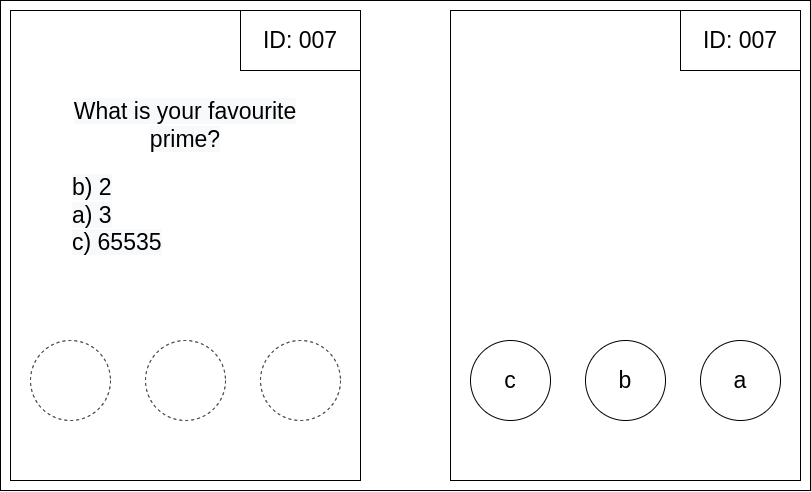
\includegraphics[width=0.7\textwidth]{../resources/high_level_ballot.drawio}
\caption{Punchscan ballot consisting of top (left) and bottom (right) page}
\label{fig:punchscan_ballot}
\end{figure}

\section{Voting process}

After having identified themselves at the polling place, a voter will have to
commit to getting to keep either the top or the bottom page of the ballot as a
receipt. They will then receive a random ballot, consisting of a top and bottom
page stuck together and enter the voting booth.

Within, the voter will read the question and decide on their answer. They will
look up which symbol their choice maps to on the top page, and then look
through which hole on the top page the corresponding symbol printed on the
bottom page is visible. They will then mark the corresponding slot using a
dauber --- a huge highlighter as used in Bingo --- thereby leaving a stain on
both the top as well as the bottom page of the ballot. The effect of having
marked their choice is shown in figure \ref{fig:punchscan_ballot_voted}.

The voter will then destroy the half of the ballot they will not keep by
feeding it through a shredder. They then exit the voting booth, and hand the
remaining half to a poll worker. The poll worker will scan the page, and feed
it through an OCR software. The voter gets to see and confirm that the scanned
page, including the detected choice, matches their physical copy. If so they
get to leave, keeping their scanned half of the ballot as a receipt.

\begin{figure}
\centering
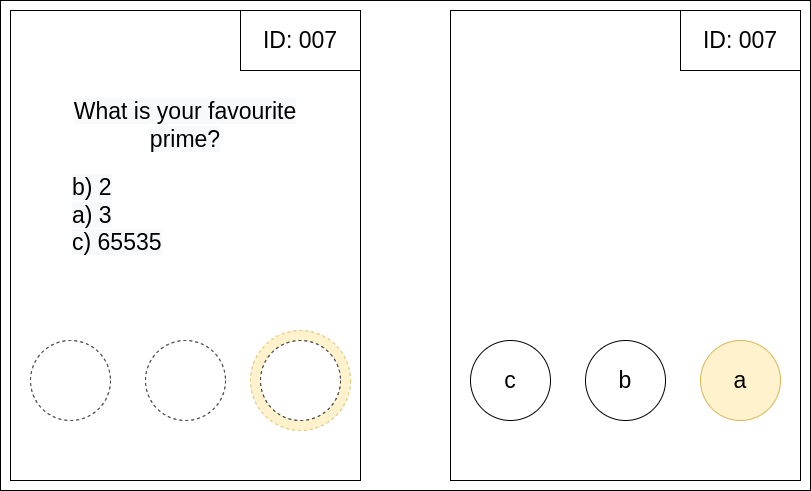
\includegraphics[width=0.7\textwidth]{../resources/high_level_ballot_voted_split.drawio}
\caption{Top (left) and bottom (right) pages of ballot after voter chose `3' as their favourite prime}
\label{fig:punchscan_ballot_voted}
\end{figure}

\chapter{Setup}
\label{ch:setup}

During the setup phase the election authority will initialize the contents of
three tables. This will be followed by an audit to ensure honesty of the
election authority. The three tables which are initialized are referred to as
the \textbf{P}, \textbf{D} and \textbf{R} tables:
\begin{description}
\item[\emph{P}rint table] The print table contains all information which is
	required to print the ballots, along with information for auditing
		purposes.
\item[\emph{D}ecryption table] The decryption table contains all information
	required to decrypt the voter's encrypted vote in the tally phase,
		along with information for auditing purposes.
\item[\emph{R}esults table] The results table contains the outcome of election.
\end{description}

For the following we will assume an election with one question and two answers
$a$ and $b$, voted on by $n$ voters.

\section{Election authority in a threshold setting}

For the purpose of this chapter we assume the election authority to be a single
entity, in full possession of their private keys. In a real-life deployment it
would be prudent to utilize some form of threshold cryptography to spread this
trust across multiple parties.

\section{Initializing the \textbf{P} table}

The election authority first populates $2n$ rows of the \textbf{P} table as shown
in table \ref{tbl:p_table_full}. This table is indexed by a primary key $ID_P$,
corresponding to the ballot ID which will be printed on both pages of the
ballot. It then picks two random permutations \ptop{} and \pbottom{},
corresponding to the permutations of the top and bottom pages respectively.
Permutations will be shown explicitly. In an actual implementation they might
however be chosen as shown in section \ref{sec:generating_permutations}. The
\emph{Choice} column is left empty, and will be used to store the voter's
permuted choice later on.

For each row it then calculates two cryptographic commitments, \ctop{} and
\cbottom{}, to \ptop{} and \pbottom{} respectively. The utilized commitment
scheme is described in section \ref{sec:commitment_scheme}.

\begin{table}
	\centering
	\begin{tabular}{|c|c|c|c|c|c|}
		\hline
		$ID_P$ & \ptop & \pbottom & $Choice$ & \ctop & \cbottom \\
		\hline
		1 & ab & ab & & $C_{1, 1}$ & $C_{1, 2}$ \\
		2 & ab & ba & & $C_{2, 1}$ & $C_{2, 2}$ \\
		3 & ba & ab & & $C_{3, 1}$ & $C_{3, 2}$ \\
		4 & ba & ba & & $C_{4, 1}$ & $C_{4, 2}$ \\
		5 & ab & ba & & $C_{5, 1}$ & $C_{5, 2}$ \\
		6 & ba & ab & & $C_{6, 1}$ & $C_{6, 2}$ \\
		\hline
	\end{tabular}
	\caption{Print table}
	\label{tbl:p_table_full}
\end{table}

\section{Initializing the \textbf{D} table}

The election authority then populates $2n$ rows of the \textbf{D} table as per
table \ref{tbl:d_table_full}. This table contains a reference to the \textbf{P}
table by means of the $ID_P$ column, and to the \textbf{R} table by means of
the $ID_R$ column. Both $ID_P$ and $ID_R$ are random and independent
permutations of the elements $1, 2, \ldots, 2n$. It then chooses \pone{}
randomly, and calculates \ptwo{} such that $\ptwo \circ \pone \circ \pbottom
\circ \ptop = id$ yields the identity permutation.  The $\hat{R}$ column is
left empty during the setup phase and will be used during decryption. 

Finally a  cryptographic commitment $Com_i$ to each row is generated, as well
as two cryptographic commitments $Com_{ID_P, \pone}$ to the content of columns
$ID_P$ and \pone{}, and $Com_{\ptwo, ID_R}$ to the content of columns \ptwo{}
and $ID_R$.

\begin{table}[h]
	\begin{subtable}{.6\linewidth}
		\centering
		\begin{tabular}{|c|c|c|c|c|c|}
			\hline
			$ID_P$ & $\pi_1$ & $\hat{R}$ & $\pi_2$ & $ID_R$ & $Com_{i}$ \\
			\hline
			6 & $\rightarrow$       & & $\circlearrowright$ & 5 & $C_6$ \\
			5 & $\circlearrowright$ & & $\rightarrow$       & 4 & $C_5$ \\
			2 & $\circlearrowright$ & & $\rightarrow$       & 1 & $C_2$ \\
			1 & $\circlearrowright$ & & $\circlearrowright$ & 3 & $C_1$ \\
			4 & $\rightarrow$       & & $\rightarrow$       & 2 & $C_4$ \\
			3 & $\rightarrow$       & & $\circlearrowright$ & 6 & $C_3$ \\
			\hline
			\multicolumn{2}{|c|}{$Com_{ID_P, \pi_1}$} &   & \multicolumn{2}{c|}{$Com_{\pi_2, ID_R}$} & \\
			\hline
		\end{tabular}
		\caption{Decryption table}
		\label{tbl:d_table_full}
	\end{subtable}%
	\begin{subtable}{.4\linewidth}
		\centering
		\begin{tabular}{|c|c|}
			\hline
			$ID_R$ & $R$ \\
			\hline
			1 & \\
			2 & \\
			3 & \\
			4 & \\
			5 & \\
			6 & \\
			\hline
			\multicolumn{2}{l}{} % Ugly hack to vertically align the two tables.
		\end{tabular}
		\caption{Results table}
		\label{tbl:r_table_full}
	\end{subtable}
	\caption{Decryption and results tables}
\end{table}

\section{Initializing the \textbf{R} table}

In a last step the election authority initializes $2n$ empty rows of the
\textbf{R} table as shown in table \ref{tbl:r_table_full}.

\begin{table}
\end{table}

\section{Setup audit}

The final phase of the setup consists of a first audit by a set of trusted
auditors. The election authority reveals the primary ballot ID $ID_P$ and
commitments of the \textbf{P} table, as well as the row and column commitments
of the \textbf{D} table. The revealed data is shown in table
\ref{tbl:setup_audit}. The auditor then gets to pick $n$ rows at random, for
which the election authority will reveal the full contents, including what is
required to open the commitments. An example of a revealed table is shown in
table \ref{tbl:setup_audit_revealed}. The auditor will then verify that all row
commitments are correct, and that $\ptwo \circ \pone \circ \pbottom \circ \ptop
= id$ holds.

All rows which were fully revealed during this audit are considered spoiled,
and will not be used anymore in subsequent parts of the voting scheme.

\begin{table}[h]
	\centering
	\begin{subtable}{.5\linewidth}
		\begin{tabular}{|c|c|c|c|c|c|}
			\hline
			$ID_P$ & $\pi_{t}$ & $\pi_{b}$ & $c$ & $Com_{\pi_{t}}$ & $Com_{\pi_{b}}$ \\
			\hline
			1 & & & & $C_{1, 1}$ & $C_{1, 2}$ \\
			2 & & & & $C_{2, 1}$ & $C_{2, 2}$ \\
			3 & & & & $C_{3, 1}$ & $C_{3, 2}$ \\
			4 & & & & $C_{4, 1}$ & $C_{4, 2}$ \\
			5 & & & & $C_{5, 1}$ & $C_{5, 2}$ \\
			6 & & & & $C_{6, 1}$ & $C_{6, 2}$ \\
			\hline
		\end{tabular}
	\end{subtable}%
	\begin{subtable}{.5\linewidth}
		\begin{tabular}{|c|c|c|c|c|c|}
			\hline
			$ID_P$ & $\pi_1$ & $\hat{R}$ & $\pi_2$ & $ID_R$ & $Com_{i}$ \\
			\hline
			& & & & & $C_6$ \\
			& & & & & $C_5$ \\
			& & & & & $C_2$ \\
			& & & & & $C_1$ \\
			& & & & & $C_4$ \\
			& & & & & $C_3$ \\
			\hline
			\multicolumn{2}{|c|}{$Com_{ID_P, \pi_1}$} &   & \multicolumn{2}{c|}{$Com_{\pi_2, ID_R}$} & \\
			\hline
		\end{tabular}
	\end{subtable}
	\caption{Subset of tables released for auditing purposes}
	\label{tbl:setup_audit}
\end{table}

\begin{table}
	\centering
	\begin{subtable}{.5\linewidth}
		\begin{tabular}{|c|c|c|c|c|c|}
			\hline
			$ID_P$ & $\pi_{t}$ & $\pi_{b}$ & $c$ & $Com_{\pi_{t}}$ & $Com_{\pi_{b}}$ \\
			\hline
			1 & & & & $C_{1, 1}$ & $C_{1, 2}$ \\
			2 & ab & ba & & $C_{2, 1}$ & $C_{2, 2}$ \\
			3 & & & & $C_{3, 1}$ & $C_{3, 2}$ \\
			4 & ba & ba & & $C_{4, 1}$ & $C_{4, 2}$ \\
			5 & ab & ba & & $C_{5, 1}$ & $C_{5, 2}$ \\
			6 & & & & $C_{6, 1}$ & $C_{6, 2}$ \\
			\hline
		\end{tabular}
	\end{subtable}%
	\begin{subtable}{.5\linewidth}
		\begin{tabular}{|c|c|c|c|c|c|}
			\hline
			$ID_P$ & $\pi_1$ & $\hat{R}$ & $\pi_2$ & $ID_R$ & $Com_{i}$ \\
			\hline
			&                     & &                     &   & $C_6$ \\
			5 & $\circlearrowright$ & & $\rightarrow$       & 4 & $C_5$ \\
			2 & $\circlearrowright$ & & $\rightarrow$       & 1 & $C_2$ \\
			&                     & &                     &   & $C_1$ \\
			4 & $\rightarrow$       & & $\rightarrow$       & 2 & $C_4$ \\
			&                     & &                     &   & $C_3$ \\
			\hline
			\multicolumn{2}{|c|}{$Com_{ID_P, \pi_1}$} &   & \multicolumn{2}{c|}{$Com_{\pi_2, ID_R}$} & \\
			\hline
		\end{tabular}
	\end{subtable}
	\caption{Subset of tables released for auditing purposes}
	\label{tbl:setup_audit_revealed}
\end{table}

\section{Generating permutations}
\label{sec:generating_permutations}

Implementations of Punchscan must be able to generate permutations in such a
way that three properties hold:
\begin{itemize}
	\item Observing parts of a permutation must give an attacker no useful information about the rest of the permutation.
	\item A compact representation must exist, such that it can be stored in a database.
	\item Permutations must be generated computationally, in a way that all
		members of the election authority trust the process.
\end{itemize}

The introductory paper outlines two ways by which such permutations can be
constructed \autocite[section 8]{fisherPunchscanIntroductionSystem2006}. The
first, shown in section \ref{sec:permutations_via_symmetric_cipher} is used to
permute the rows of the $D$ and $R$ tables. The second, shown in section
\ref{sec:permutations_via_shifts} is used to permute the top and bottom pages
of the ballot.

\subsection{Generate permutation over $n$ elements using a symmetric cipher}
\label{sec:permutations_via_symmetric_cipher}

Agree on a symmetric cipher and key $K$. Start with a table with two columns.
Initialize the first column to values $1, 2, \ldots, n$. Fill the second column
with $Enc_K(1), Enc_K(2), \ldots, Enc_K(n)$, where $Enc_K(i)$ is the result of
encrypting $i$ with key $K$ --- using a standard padding scheme if required.
Sort the table by the second column using some canonical ordering. Then, the
order of the numbers in the first column defines a permutation
indistinguishable from a truly random permutation, given standard assumptions
placed on symmetric ciphers.

\subsection{Generate permutation over $n$ elements as combination of two cyclic shifts}
\label{sec:permutations_via_shifts}

For the $\pi_1, \pi_2, \pi_{top}, \pi_{bottom}$ permutations the authors note
that a simpler consruction is sufficient to generate all possible mappings
between answer possibilities and symbols. They propose to generate two random
numbers, and cyclically shift the list of answer possibilities by one of the
random numbers, and the list of answer symbols by the other. This will not
generate all possible permutations as e.g. the relative order of elements is
preserved.

\section{Commitment scheme}

The introductory paper defines their own custom commitment scheme based on the
AES block cipher\autocite[section 9]{fisherPunchscanIntroductionSystem2006}.
Let $K_1, K_2$ be two AES-128 keys. Let $C$ be a public 128-bit constant. Let
$Enc_K(m)$ denote the result of encrypting a 128-bit message $m$ using the key
$K$, $Dec_K(c)$ the result of decrypting a 128-bit ciphertext $c$ using the key
$K$. Let $||$ denote binary concatenation.

\subsection{Key-derivation function}

They first define a custom key-derivation function, shown in algorithm
\ref{alg:kdf}.

\begin{algorithm}
	\begin{algorithmic}
		\State \textbf{Input} $m$
		\State $m_{128} \gets \text{First 128 bits of } m$ \Comment{Pad with zeroes if $m$ shorter than 128 bits}
		\State $K_m \gets Dec_{K_1}(C \oplus Enc_{K_2}(C \oplus Enc_{K_1}(m_{128})))$
		\State \textbf{Return} $K_m$
	\end{algorithmic}
	\caption{$KDF(m)$}
	\label{alg:kdf}
\end{algorithm}

\subsection{Commitment scheme}

They then define a commitment scheme as shown in algorithm \ref{alg:commit}.

\begin{algorithm}
	\begin{algorithmic}
		\State \textbf{Input} $m$
		\State $K_m \gets \Call{KDF}{m}$
		\State $s \gets Enc_{K_m}(C)$
		\State $h_1 \gets \Call{SHA-256}{m || s}$
		\State $h_2 \gets \Call{SHA-256}{m || Enc_{K_m}(h_1)}$ \Comment{AES in ECB mode with PKCS\#5 padding}
		\State \textbf{Return} $(h_1, h_2)$
	\end{algorithmic}
	\caption{$Commit(m)$}
	\label{alg:commit}
\end{algorithm}

\subsection{Opening commitments}

While not described in the paper, one can surmise that opening the commitments
is done by releasing $K_m$. As generation of commitments is deterministic, this
will allow recalculating the commitment and comparing for equality.

\chapter{Vote decryption and tallying}

Recall that during the voting process one half of the ballot was scanned. The
voter's choice is stored in the \emph{Choice} column of the \emph{P} table. It
is represented either as a number, indicating which of the fields (in some
canonical order) the voter selected, or as an actual choice under the
assumption that the voter had had a `canonical' ballot --- that is a ballot
with $\ptop = \pbottom = id$. In the decryption phase this permuted choice is
then transformed into the plaintext choice in an auditable way.

\section{Decrypting the vote}

Assume that the voter's plaintex choice was $m$. Then the voter's recorded
choice is equal to $Choice = (\ptop{} \circ \pbottom{})(m)$. In a first step
the election authority calculates $\hat{R} = \pone{}(Choice)$, and $R =
\ptwo{}(\hat{R})$. Thus $R = (\ptwo \circ \pone \circ \pbottom \circ \ptop)(m)
= id(m) = m$, so the decrypted vote is correct. The election authority can then
tally the plaintext votes and publish the results.

\section{Decryption audit}

Similarly to the setup audit, the election authority again publishes a subset
of the \emph{P}, \emph{D} and \emph{R} tables as shown in table
\ref{tbl:decryption_audit}. The auditor then gets to decide which half of the
\emph{D} table to reveal. If they choose the left half then $ID_P$ and \pone{}
gets revealed, otherwise $ID_R$ and \ptwo{}. The auditor then checks that the
appropriate relation between $Choice$, $\hat{R}$ and $R$ holds, and that the
appropriate column commitment holds.

\begin{table}
	\centering
	\begin{subtable}{.2\linewidth}
	\end{subtable}%
		\centering
		\begin{tabular}{|c|c|}
			\hline
			$ID_P$ & $C$ \\
			\hline
			1 & a \\
			3 & b \\
			6 & a \\
			\hline
		\end{tabular}
	\begin{subtable}{.6\linewidth}
		\centering
		\begin{tabular}{|c|c|c|c|c|}
			\hline
			$ID_P$ & $\pi_1$ & $\hat{R}$ & $\pi_2$ & $ID_R$ \\
			\hline
			  &                     & a &                     &   \\
			  &                     & b &                     &   \\
			  &                     & b &                     &   \\
			\hline
			\multicolumn{2}{|c|}{$Com_{ID_P, \pi_1}$} &   & \multicolumn{2}{c|}{$Com_{\pi_2, ID_R}$} \\
			\hline
		\end{tabular}
	\end{subtable}
	\begin{subtable}{.2\linewidth}
		\centering
		\begin{tabular}{|c|c|}
			\hline
			$ID_R$ & $R$ \\
			\hline
			3 & a \\
			5 & b \\
			6 & a \\
			\hline
		\end{tabular}
	\end{subtable}
	\caption{Subset of tables released for auditing purposes}
	\label{tbl:decryption_audit}
\end{table}

\subsection{Lowering success chance of a cheating election authority}

To improve resiliency, the \emph{D} table can be split into independent shards
containing $k$ rows each, each with their own column commitments. During
auditing, the auditor can then choose, for each shard, which half to reveal.

\section{Individual verifiability}

As a last step the election authority publishes the list of scanned ballot
halves, corresponding to the $Choice$ column of the \emph{P} table. This allows
each voter to then look up their ballot using its ID, and compare that the
scanned image matches their physical receipt.

\chapter{Privacy and security}
\label{ch:security}

Punchscan intends to provide two measures of security: Voters' privacy and vote
integrity. This chapter will show to what extend it succeeds in doing that, and
what its limitations are.

\section{Voter privacy}

Voter privacy is essential to prevent a malicious third party from buying, or
coercing, voters. It is clear that privacy can not be guaranteed by the voting
system alone: Consider the case of a voter filming themselves during the voting
process. However a voting system should be able to ensure that, after the
voting process, a voter's privacy cannot be violated anymore. Other risks to
voter privacy would have to be addressed by regulations, such as not
permitting the use of video-capturing devices in voting booths.

\subsection{Privacy against a malicious election authority}

Punchscan does not achieve any form of privacy against a malicious election
authority. Having full access to the \textbf{P} table means that they can
reconstruct any voter's plaintext vote. Assuming voting booth workers to be
compromised, this then leaks every voter's vote.

\subsection{Privacy against third parties}

After having voted, a voter is left with one half of the ballot. A third party
will then, at most, have access to the following:
\begin{itemize}
\item For every ballot, either \ptop{} or \pbottom{} due to the scanned receipts being published along with their ballot ID
\item For each shard of the \textbf{D} table, either the \pone{} or the \ptwo{}
permutations
\item For each shard of the \textbf{D} table, either the $ID_P$ link to the
\textbf{P} table, or the $ID_R$ link to the \textbf{R} table
\item The full results table
\end{itemize}

Thus they will, for any given ballot, be lacking one of the ballot
permutations, one of the decryption permutations, and one of the chain of
mappings from \textbf{P} to \textbf{D} to \textbf{R} tables. Hence they will not be
able to learn the plaintext vote of any ballot.

\subsection{Vote-buying attack}

There does however exist a vote-buying attack on an earlier version of
punchscan, described by Moran and
Naor\autocite{moranSplitballotVotingEverlasting2010}. The key difference is
that this earlier version of Punchscan did not require a voter to commit to
which half of the ballot to keep until after they had voted. It can be shown
that a coercing party can pick a subset of receipts for which they are willing
to pay in such a way as to influence the election outcome.

For illustration purposes consider a vote between two candidates, Alice and
Bob. There will be two choices for \ptop{}, two for \pbottom{}, leading to four
different ballots. Assume the coercing party wants to influence the vote in
favour of Alice. Assume they state that they will pay for any ballot receipt,
as long as:
\begin{itemize}
\item It is not a ballot where the order of options is $b \rightarrow a$
\item And the voter did not selection the second option
\end{itemize}

The four possible ballots, with their respective ballot halves, are shown in
figure \ref{fig:vote_buying}. Green ballot halves are those with order $a
\rightarrow b$, so a voter will receive payment no matter who they vote for.
Orange ones are $b \rightarrow a$ receipts, so the voter must pick the left
option --- voting for Bob --- if they want to get paid. Red ones are $b
\rightarrow a$ receipts, so the voster must vote for Alice in order to get paid.
Thus the coercing party is able to force one out of four Bob voters to vote for
Alice, without causing any Alice voters to vote for Bob.

The same attack is also shown to be extensible to questions with more than two
votes. The fix for Punchscan is straight-forward, requiring voters to commit to
which half of the ballot to keep before they get access to the ballot. This way
the coercing party will also inadvertently pay Alice voters to vote for Bob
instead.

\begin{figure}
\centering
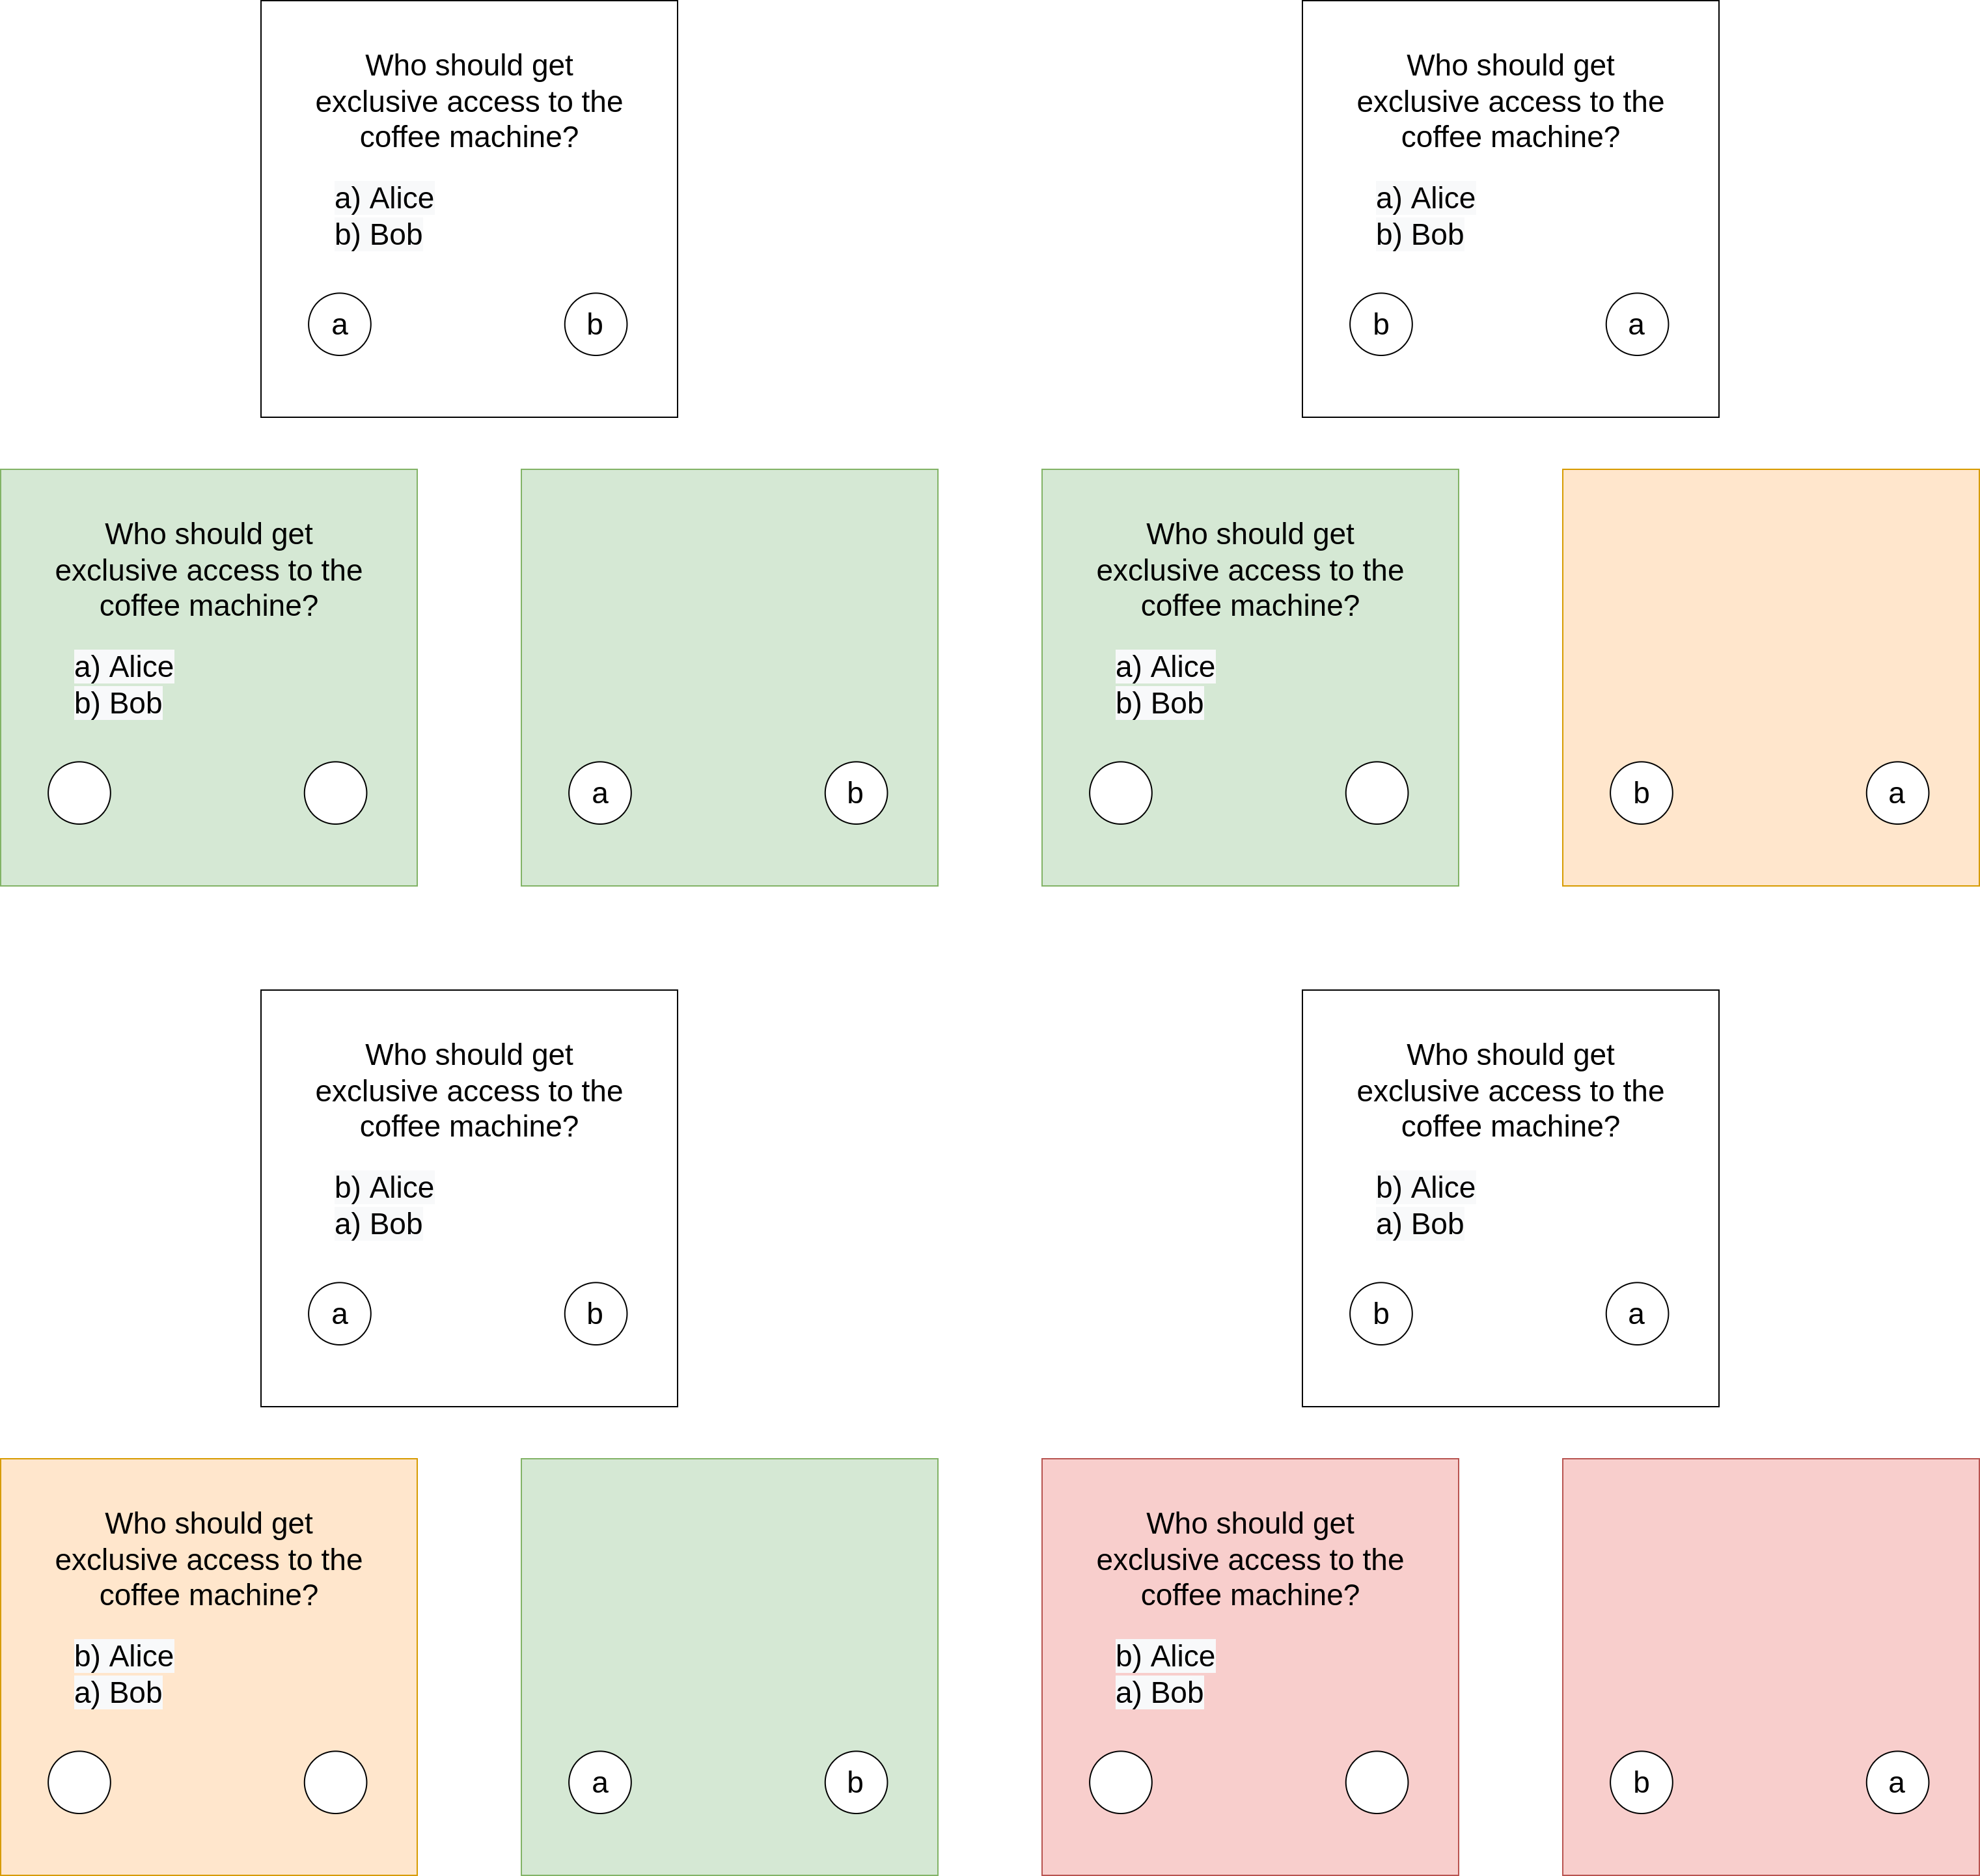
\includegraphics[width=0.8\textwidth]{../resources/vote_buying_split_highlighted_no_selection.drawio.png}
\caption{Green ballot halves allow getting paid no matter who you vote for. Orange ones require voting for Bob. Red ones require voting for Alice.}
\label{fig:vote_buying}
\end{figure}

\section{Vote integrity}

Punchscan provides some form of vote integrity versus a malicious election
authority --- at least during the setup and decryption phases.

\subsection{Setup-phase audit}

Recall that during the setup phase a certain number of rows of the \textbf{P} and
\textbf{D} tables are spoiled and verified. Thus for every row where the election authority 
was dishonest there is a chance of $\frac{1}{2}$ of it being caught. Consider the
generalized case where the election authority cheats on $f$ out of $n$ ballots,
with $k$ being audited. The introductory paper shows that an upper bound of the
election authority not being caught is given by:

\[
	[(1 - \frac{k}{n})^f, (1 - \frac{f}{n})^k]
\]

This bound can be made arbitrarily small by increasing the ratio of audited
ballots to total ballots.

\subsection{Decryption-phase audit}

Recall that during decryption one half of each shard of the \textbf{D} table is
revealed. To minimze its chance of being caught, a cheating election authority
will spread the votes on which it cheated across as few shards as possible.
Assuming $k$ shards were tempered with then this audit has a chance of
$\frac{1}{2^k}$ of not detecting this. Both this probability, as well as the
signifiance (in terms of tampered-with votes) of a single tampered-with shard
not being caught, can be lowered by decreasing the shard size. In the extreme
case one picks a shard size of $1$, at which points $k$ tampered votes have a
probability of $\frac{1}{2^k}$ of not being detected.

\subsection{Individual verifiability}

As the election authority publishes all scanned ballot receipts, any voter can
subsequently look up their receipt using their ballot ID. They can then compare
the scanned image with their physical receipt. This guarantees them that their
vote was at least cast-as-intended, although it does not ensure that it was
actually counted --- for this they must rely on the auditors having done their
job.

\subsection{Ballot misprinting}

One issue not addressed by Punchscan is the one of ballot integrity.
Fundamentally one must ensure that the printed ballots correspond to the the
remainders of the \textbf{P} table after the setup audit. The Punchscan paper
advises that voters should, the moment they receive the ballot, verify that
their ballot's commitment matches one of the published commitments. They do not
however provide any way in which a voter --- equipped with pen and paper ---
can do so in the few minutes they spend in a voting booth.

An alternative might be to introduce an additional audit phase, during which a
fraction of printed ballots is audited. The remaining unspoiled ballots would
then be sealed by the auditors, and not reopened until the day of the election.
No discussion of this takes place in the Punchscan paper, but Kelsyey et
al\autocite{kelseyAttackingPaperBasedE2E2010} mention it in passing.

\subsection{Malicious poll workers}

Kelsey et al also discuss a specific misprinting attack on
Punchscan\autocite[chapter 3]{kelseyAttackingPaperBasedE2E2010} where, when a
voter announced which half of the ballot they intend to keep, the poll worker
hands them a ballot where the half which will be destroyed is manipulated. As
discussed the voter is unable to verify the commitments in the voting booth.
When they then leave the voting booth, the only evidence of having cheated ---
the manipulated half of the ballot --- is destroyed. To prevent this one would
have to make poll workers commit to which ballot to hand out before the voter
announces which page to keep. At the same time one must still ensure that a
voter does not see their future ballot until after they commited to which half
to keep. Even more ways by which a cheating election authority can influence
the vote are discussed by Lundin et al\autocite{lundinTearDestroyChain2012}.

\section{Attacking cryptographic primitives}

The Punchscan paper goes into some detail to discuss potential attacks on the
cryptographic primitives they use for e.g. row commitments or the generation of
permutations. This will not be discussed here, as the security assumptions
placed on basic cryptographic primitives are assumed to hold.

\chapter{Conclusion}

Punchscan has shown that using cryptographic operations allows one to work with
weaker trust assumptions, such as a potentially malicious election authority.
It has however suffered from a variety of attacks and other weaknesses during
its --- rather short --- life. It thus also serves to highlight the importance
of formalising security proofs and assumptions.

Punchscan did have the advantage that its workings are relatively
straight-forward, and could be explained well to non-technical people. While
more recent electronic voting systems offer more in terms of security against
malicious parties or verifiability, they achieve this by added layers of
complexity which prevent the vast majority of people from getting more than a
cursory understanding of how they work.


\printbibliography

\end{document}
